\section{The Heston Model}

\subsection{Model Description}

- Von Heston (1993) vorgestellt und ist ein stochastic volatility model, die Volatilität ist nicht konstant, wie z.B. beim Black-Scholes-Merton-Model, sondern folgt auch einem random process.
\begin{align}
    \label{eq:heston_model_price}
    \mathrm{d}S_t &= \mu S_t\mathrm{d}t + \sqrt{v_t}S_t\mathrm{d}W_t^S \\
    \label{eq:heston_model_log_price}
    \mathrm{d}X_t = \mathrm{d}\log(S_t) &= \left(\mu-\frac{1}{2}v_t\right)\mathrm{d}t + \sqrt{v_t}\mathrm{d}W_t^S \\
    \label{eq:heston_model_variance}
    \mathrm{d}v_t &= \kappa(\theta-v_t)\mathrm{d}t + \sigma\sqrt{v_t}\mathrm{d}W_t^v \\
    \label{eq:heston_model_correlation}
    \mathbb{E}(\mathrm{d}W_t^S\mathrm{d}W_t^v) &= \rho\mathrm{d}t
\end{align}
wobei $\kappa$, $\theta$ und $\sigma$ strikt positiv sind, $\mathrm{d}W_t^S$ und $\mathrm{d}W_t^v$ sind increments von Brownian Motions mit der Korrelation $\rho$. $S_t$ ist der Preis eines Assests, z.B. einer Aktie, Aleihe, FX-Rate, etc. Der Prozess $X_t$ ist der Logarithmus des Preisprozesses $S_t$; $v_t$ ist der instantaneous Varianz-Prozess. Der Parameter $\mu$ ist der Drift des Preis-Prozesses.

- Varianz-Prozess ist ein CIR-Process (Cox-Ingersoll-Ross, Cox et al 1985) mit Mean-Reversion $\kappa$, Long-Run-Varianz $\theta$ und Volatilität $\sigma$. Die Übergangswahrscheinlichkeit von $v_t$ conditional on $v_0$ ist proportional zu einer noncentral chi-squared verteilten Zufallsvariable:
\begin{align}
    \label{eq:heston_model_variance_transition}
    v_t\mid v_0 &\sim c\cdot \chi^2'_{\nu}(\Lambda) \\
    c &= \sigma^2\left(1 - \exp(-\kappa t)\right)(4\kappa)^{-1} \notag \\
    \nu &= \frac{4\kappa\theta}{\sigma^2} \notag \\
    \Lambda &= \frac{v_0}{c}\exp(-\kappa t) \notag
\end{align}
$\chi^2'$ steht für eine nichtzentrale Chi-Quadrat-Verteilung mit $\nu$ Freiheitsgraden und $\Lambda$ als nichtzentralem Parameter (Okhrin et al 2022).

\subsection{Characteristic Function and Density of the Heston Model}
- Hat eine Zufallsvariable $X$ eine Dichte $f(x)$, so kann man die charakteristische Funktion $\phi(t)$ von $X$ berechnen durch
\begin{align}
    \phi(t) = \mathbb{E}(\exp(\mathrm{i}tX)) = \int_{-\infty}^{\infty} e^{\mathrm{i}tx}f(x)\mathrm{d}x \notag
\end{align}
- Die charakteristische Funktion für eine Zufallsvariable existiert immer, auch wenn die Dichte nicht existiert. Hat man die charakteristische Function, so kann man die Dichte durch die inverse Fourier-Transformation berechnen
\begin{align}
    f(x) = \frac{1}{2\pi}\int_{-\infty}^{\infty} e^{-\mathrm{i}tx}\phi(t)\mathrm{d}t \notag
\end{align}
- Gatheral (2011) hat die charakteristische Funktion des Heston-Modells berechnet
\begin{align}
    \phi(t) = \exp(A + B + C) \notag
\end{align}
mit
\begin{align}
    A &= \mu\cdot\tau\cdot t\cdot\mathrm{i} \notag \\
    d &= \sqrt{(\rho\sigma\mathrm{i}t - \kappa)^2 - \sigma^2(-\mathrm{i}t - t^2)} \notag \\
    g &= \frac{\kappa - \rho\sigma\mathrm{i}t - d}{\kappa - \rho\sigma\mathrm{i}t + d} \notag \\
    B &= \frac{\theta\kappa}{\sigma^2}\left(\tau(\kappa - \rho\sigma\mathrm{i}t - d) - 2\log\left[\frac{1-g\exp(-d\tau)}{1-g}\right]\right) \notag \\
    \gamma &= \frac{2\kappa\theta}{\sigma^2} \notag \\
    \label{eq:heston_model_characteristic_function_C}
    C &= \log\left(\left[\frac{2\kappa}{\sigma^2}\right]^{\gamma}\cdot \left\lbrace \frac{2\kappa}{\sigma^2} - \frac{\kappa - \rho\sigma\mathrm{i}t - d}{\sigma^2}\cdot\frac{1 - \exp(-d\tau)}{1-g\exp(-d\tau)} \right\rbrace^{-\gamma}\right)
\end{align}
und $\tau = T-t$ als Zeithorizont.
- Eine simple inverse Fourier-Transformation ist nicht sinnvoll, da es zu numerischen Instabilitäten an den Rändern kommt (siehe \ref{fig:ifft_comparison}). Bei der simplen Methode wird $\phi(t)$ zentiert und $f(x)$ mit der Schrittweite $\Delta t$ normiert um korrekte Amplituden zu erhalten. Die andere Methode verwendet eine Randkorrektur, was die Rekonstruktion der Dichte verbessert. Zudem werden die Ergebnisse durch eine kubische Spline-Interpolation geglättet.
- Die Formel \eqref{heston_model_characteristic_function_C} hat das Problem, dass sie zu overflow Fehlern führen kann, da der Term $\left(\frac{2\kappa}{\sigma^2}\right)^\gamma$ sehr groß werden kann und der Logarithmus dann nicht mehr gezogen werden kann. Daher wird die Formel umgeschrieben:
\begin{align}
    \label{eq:heston_model_characteristic_function_C_2}
    C_{unc} = \gamma \log\left(\frac{2\kappa}{\sigma^2}\right) - \gamma \log\left(\frac{2\kappa}{\sigma^2} - \frac{\kappa - \rho\sigma t \mathrm{i} - d}{\sigma^2} \frac{1 - \exp(-d \tau)}{1 - g \exp(-d \tau)}\right)
\end{align}

\begin{figure}[h]
    \centering
    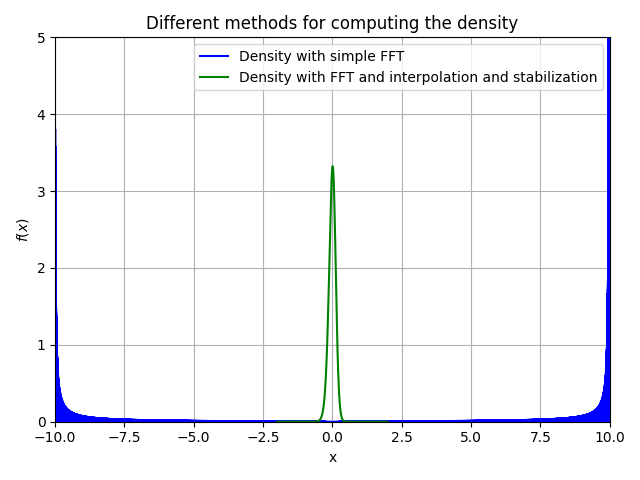
\includegraphics[width=0.8\textwidth]{img/different_ifft_methods.png}
    \caption{Comparison of different methods for the inverse Fourier transformation of the characteristic function of the Heston model ($\mu=0$, $\kappa=3$, $\theta=0.19$, $\sigma=0.4$, $\rho=-0.7$, $\tau=\frac{1}{12}$). Grid points: $N=2^{15}$}
    \label{fig:ifft_comparison}
\end{figure}

\subsection{Simulating the Heston Model}

- Heston Model is a model with continuous time, for simulation we need to discretize the time. Small timesteps require a lot of computational power, large timesteps can lead to zero or negative volatility if the so called Feller condition is not satisfied (Albrecher et al 2007). The Feller condition is satisfied if $2\kappa\theta > \sigma^2$ but Eraker et al (2003) show, that for S&P 500 index options the Feller condition is not satisfied. There are many more studies that show this result for other markets and assets (e.g. Chang et al 2021, Hu & Liu 2022).
- Intuitivster Weg der Zeit-Diskretisierung: Euler–Maruyama Diskretisierung:
\begin{align}
    X_{t+\Delta} &= X_t - \frac{1}{2}v_t\Delta + \sqrt{v_t}\sqrt{\Delta}Z_{X,t} \notag \\
    v_{t+\Delta} &= v_t + \kappa(\theta - v_t)\Delta + \sigma\sqrt{v_t}\sqrt{\Delta}Z_{v,t} \notag
\end{align}
wobei $Z\sim\mathcal{N}(0,1)$, $\Delta = T/n$, $T$ die gesamte Zeit und $n$ die Anzahl der Schritte ist. Die Korrelation zwischen $Z_{X,t}$ und $Z_{v,t}$ kann man wie folgt simulieren (Andersen 2008): %TODO: andere Quelle finden, nicht immer nur Andersen oder Ostap
\begin{align}
    Z_{v,t} &= \Phi^{-1}(U_1) \notag \\
    Z_{X,t} &= \rho Z_{v,t} + \sqrt{1-\rho^2}\Phi^{-1}(U_2) \notag
\end{align}
wobei $U_1$ und $U_2$ unabhängige Zufallsvariablen sind, die gleichverteilt sind auf $[0,1]$ und $\Phi^{-1}$ die inverse Verteilungsfunktion der Standardnormalverteilung ist.
- Bei dieser Diskretisierung sieht man auch gut das Problem der möglichen Negativität der Volatilität (Okhrin et al 2022):
\begin{align}
    \mathbb{P}(v_{t+\Delta}<0 \mid v_t>0) &= \mathbb{P}\left(Z_{v,t} < \frac{-v_t-\kappa(\theta-v_t)\Delta}{\sigma\sqrt{v_t}\sqrt{\Delta}}\right) \notag \\
    &= \Phi\left(Z_{v,t} < \frac{-v_t-\kappa(\theta-v_t)\Delta}{\sigma\sqrt{v_t}\sqrt{\Delta}}\right) \notag \\
    &> 0 \notag
\end{align}
wobei $\Phi$ die Verteilungsfunktion der Standardnormalverteilung ist. Es gibt verschiedene Methoden, um dieses Problem zu lösen, z.B. die Absorption (replace $v_t$ mit $v_t^+ = \max{0, v_t}$) oder Reflection Method (replace $v_t$ mit $\vert v_t\vert$). Alle diese Methoden ändern aber den unterliegenden Prozess, daher stimmen z.B. die Momente der Volatilität nicht mehr mit den theoretischen Momenten überein (Okhrin et al 2022, Tsoskounoglou 2024). 
- In der Studie von Okhrin et al (2022) Andersen's QE scheme performs best in terms of speed and accuracy. Andersen (2008) approximates the noncentral chi-square distribution in \eqref{eq:heston_model_variance_transition} with a mixture of distributions, a Dirac distribution and a noncentral Gaussian distribution. Für ausreichend große Werte von $v_t$ gilt
\begin{align}
    \label{eq:qe_normal}
    v_{t+\Delta} = a(b+Z_v)^2
\end{align}
mit $Z_v\sim\mathcal{N}(0,1)$. Für andere Werte von $v_t$ gilt
\begin{align}
    \label{eq:qe_dirac}
    v_{t+\Delta} &= \Psi^{-1}(U_v, p, \beta) \\
    \Psi^{-1}(u,p,\beta) &= \begin{cases}
        0 & 0\le u\le p \\
        \beta^{-1}\ln\left(\frac{1-p}{1-u}\right) & p<u\le 1
    \end{cases} \notag
\end{align}
Die Parameter $a$, $b$, $p$ und $\beta$ werden über moment-matching geschätzt, vom dem einen zum anderen Schema kann man wechseln, wenn der Wert $\psi$ über einer Schelle $\psi_c$ liegt. Dann nutzt man \eqref{eq:qe_dirac}, sonst \eqref{eq:qe_normal}. Der Wert $\psi$ ist der Quotient aus $s^2$ und $m^2$, wobei $m$ der Erwartungswert von $v_{t+\Delta}$ und $s^2$ die Varianz von $v_{t+\Delta}$ ist.
- Für den Preisprozess schlägt Andersen (2008) folgendes Schema vor:
\begin{align}
    \ln(S_{t+\Delta}) &= \ln(S_t) + K_0 + K_1v_t + K_2v_{t+\Delta} + \sqrt{K_3v_t + K_4v_{t+\Delta}}\cdot Z \notag \\
    K_0 &= -\frac{\rho\kappa\theta}{\sigma}\Delta \notag \\
    K_1 &= \xi_1\Delta\left(\frac{\kappa\rho}{\sigma} - \frac{1}{2}\right)-\frac{\rho}{\sigma} \notag \\
    K_2 &= \xi_2\Delta\left(\frac{\kappa\rho}{\sigma}-\frac{1}{2}\right)+\frac{\rho}{\sigma} \notag \\
    K_3 &= \xi_1\Delta(1-\rho^2) \notag \\
    K_4 &= \xi_2\Delta(1-\rho^2) \notag
\end{align}
wobei $Z$ standardnormalverteilt ist und $\xi_1$ und $\xi_2$ gewisse Konstanten sind, im Paper wird $\xi_1=\xi_2=0.5$ vorgeschlagen.